% ============================================================
% 第0章 高一必备基础回顾（必修一、必修二中理解后续内容所必需的部分）
% ============================================================
% 本章宏：电子式画法（前缀 czero）
% \czeroSide{代码}{x}{y}{h/v}：0 无，1 一个“·”电子，2 一对电子，3 一个“×”电子
\newcommand{\czeroSide}[4]{%
  \ifcase#1\relax
  \or \fill (#2,#3) circle (0.028);
  \or \if#4h\fill ({#2-0.065},#3) circle (0.028) ({#2+0.065},#3) circle (0.028);%
      \else\fill (#2,{#3-0.065}) circle (0.028) (#2,{#3+0.065}) circle (0.028);\fi
  \or \node[inner sep=0pt,font=\scriptsize] at (#2,#3) {$\times$};
  \fi}
% \czeroAt{x}{y}{元素符号}{上}{右}{下}{左}
\newcommand{\czeroAt}[7]{%
  \node[inner sep=0pt] at (#1,#2) {#3};
  \czeroSide{#4}{#1}{#2+0.25}{h}\czeroSide{#5}{#1+0.28}{#2}{v}%
  \czeroSide{#6}{#1}{#2-0.25}{h}\czeroSide{#7}{#1-0.28}{#2}{v}}
% \czeroBr{左x}{右x}{电荷}：离子的方括号
\newcommand{\czeroBr}[3]{%
  \draw (#1+0.07,0.38)--(#1,0.38)--(#1,-0.38)--(#1+0.07,-0.38);
  \draw (#2-0.07,0.38)--(#2,0.38)--(#2,-0.38)--(#2-0.07,-0.38);
  \node[anchor=west,inner sep=1pt,font=\scriptsize] at (#2,0.42) {#3};}

\chapter{高一必备基础回顾}

选择性必修的内容建立在高一化学之上：第1章计算反应热要用物质的量；第3、4章讨论化学平衡、电离和水解，要会写离子方程式；第5章电化学的核心是氧化还原反应中的电子转移；第6～8章的物质结构从原子结构和化学键讲起。本章把这四部分内容重新梳理一遍，重点放在“为什么这样规定”和“怎样用”上。对某一节已经很熟的同学，可以先做章末 A 组练习自测，做错了再回来读对应的部分。元素化合物知识放在第13章，实验基本操作放在第12章，这里不展开。

\section{物质的量}

\subsection{为什么要引入物质的量}
化学反应是按微粒个数进行的。\ce{2H2 + O2 = 2H2O} 表示 2 个氢分子与 1 个氧分子反应生成 2 个水分子。可是分子、原子极小，一滴水里就有约 $1.7\times10^{21}$ 个水分子，实验中不可能一个一个去数，只能称质量、量体积。\textbf{物质的量}（符号 $n$，单位 mol）就是把“微粒个数”与“质量、体积”联系起来的物理量。

可以拿生活中的计数单位打比方：文具店按“打”卖铅笔，一打是 12 支，说“3 打”就知道是 36 支。1 mol 所含指定微粒的数目严格规定为 $6.02214076\times10^{23}$。\textbf{阿伏加德罗常数}记作 $N_\text{A}=6.02214076\times10^{23}$ mol$^{-1}$，高中计算通常取 $6.02\times10^{23}$ mol$^{-1}$。说“1 mol”时必须说明微粒种类，例如 1 mol 氧原子与 1 mol 氧分子不是同一份物质。按高中计算精度，1 mol 微粒的质量以 g 为单位时，数值上等于它的相对原子质量或相对分子质量，例如 1 mol \ce{H2O} 的质量是 18 g。单位物质的量的物质所具有的质量叫\textbf{摩尔质量}（$M$），\ce{H2O} 的摩尔质量是 18 g·mol$^{-1}$。

气体还有一个特点。同温同压下，1 mol 不同气体的体积几乎相同，而 1 mol 不同固体或液体的体积各不相同。原因在于：常见低压气体的分子间距远大于分子本身的大小，可以近似忽略分子体积和分子间作用力；同温同压下，体积主要由分子数目决定。固体、液体中微粒紧密排列，体积还显著受到微粒大小、间距及排列方式的影响，所以没有统一的摩尔体积。单位物质的量的气体所占的体积叫\textbf{气体摩尔体积}（$V_\text{m}$）。在\textbf{标准状况}（0 ℃、101 kPa）下，$V_\text{m}\approx22.4$ L·mol$^{-1}$。

\begin{gainian}[以物质的量为中心的换算]
\[n=\frac{N}{N_\text{A}}=\frac{m}{M}=\frac{V(\text{气体})}{V_\text{m}}=c\cdot V(\text{溶液})\]
其中物质的量浓度 $c=\dfrac{n(\text{溶质})}{V(\text{溶液})}$，单位 mol·L$^{-1}$。
\end{gainian}

这几个关系可以画成图~\ref{fig:00-nmap}。读图时注意：从外圈的量走向中心的 $n$ 用除法，从 $n$ 走向外圈的量用乘法；外圈任意两个量之间的换算都要经过 $n$。例如已知气体质量求标准状况下的体积，先除以 $M$ 得到 $n$，再乘以 $V_\text{m}$。

\tu{\begin{tikzpicture}[font=\small,
  c0box/.style={draw,rounded corners=2pt,minimum width=2.2cm,minimum height=0.65cm,align=center},
  c0arr/.style={-{Stealth[length=2mm]},thick}]
\node[c0box,fill=lightblue] (n) at (0,0) {物质的量 $n$};
\node[c0box] (m) at (-4.2,0) {质量 $m$};
\node[c0box] (N) at (4.2,0) {微粒数 $N$};
\node[c0box] (V) at (0,1.9) {气体体积 $V$};
\node[c0box] (c) at (0,-1.9) {物质的量浓度 $c$};
\draw[c0arr] ([yshift=4pt]m.east)--node[above]{$\div M$}([yshift=4pt]n.west);
\draw[c0arr] ([yshift=-4pt]n.west)--node[below]{$\times M$}([yshift=-4pt]m.east);
\draw[c0arr] ([yshift=4pt]n.east)--node[above]{$\times N_\text{A}$}([yshift=4pt]N.west);
\draw[c0arr] ([yshift=-4pt]N.west)--node[below]{$\div N_\text{A}$}([yshift=-4pt]n.east);
\draw[c0arr] ([xshift=-8pt]V.south)--node[left]{$\div V_\text{m}$}([xshift=-8pt]n.north);
\draw[c0arr] ([xshift=8pt]n.north)--node[right]{$\times V_\text{m}$}([xshift=8pt]V.south);
\draw[c0arr] ([xshift=-8pt]c.north)--node[left]{$\times V(\text{溶液})$}([xshift=-8pt]n.south);
\draw[c0arr] ([xshift=8pt]n.south)--node[right]{$\div V(\text{溶液})$}([xshift=8pt]c.north);
\end{tikzpicture}}{以物质的量为中心的换算关系（$V_\text{m}$ 只用于气体）\label{fig:00-nmap}}

\begin{liti}[基础]
(1) 8.8 g \ce{CO2} 的物质的量是多少？含多少个氧原子？在标准状况下的体积是多少？(2) 将 4.0 g NaOH 溶于水配成 250 mL 溶液，求 $c(\ce{NaOH})$。
\tcblower
\jie (1) $M(\ce{CO2})=44$ g·mol$^{-1}$，$n=\dfrac{8.8\ \text{g}}{44\ \text{g·mol}^{-1}}=0.20$ mol。每个 \ce{CO2} 分子含 2 个氧原子，氧原子为 0.40 mol，即 $0.40N_\text{A}\approx2.4\times10^{23}$ 个。标准状况下 $V=0.20\ \text{mol}\times22.4\ \text{L·mol}^{-1}=4.48$ L。\\
(2) $n(\ce{NaOH})=\dfrac{4.0}{40}=0.10$ mol，$c=\dfrac{0.10\ \text{mol}}{0.250\ \text{L}}=0.40$ mol·L$^{-1}$。注意浓度公式中的 $V$ 是溶液的体积，不是所加水的体积。
\end{liti}

同温同压下，相同体积的任何气体含有相同数目的分子，这就是阿伏加德罗定律，即同温同压下 $\dfrac{V_1}{V_2}=\dfrac{n_1}{n_2}$。由此还可以推出：同温同容下 $\dfrac{p_1}{p_2}=\dfrac{n_1}{n_2}$。第3章在恒容容器中用“压强变化”判断“气体物质的量变化”，依据就是这一关系。

\subsection{阿伏加德罗常数的判断}
以 $N_\text{A}$ 为载体的选择题常把物质的量、结构和反应联系起来。这类题不仅考计算，还要求沿着图~\ref{fig:00-nmap} 的换算链，检查每一步是否成立。表~\ref{tab:00-na} 归纳了常见的检查角度。

\begin{center}
\small
\captionof{table}{判断 $N_\text{A}$ 说法的常见检查角度\label{tab:00-na}}
\begin{tabularx}{\linewidth}{p{2.4cm}X}
\toprule
检查角度 & 典型情况（$N_\text{A}$ 为阿伏加德罗常数的值） \\
\midrule
能否用 22.4 L·mol$^{-1}$ & 只适用于标准状况下的气体。标准状况下 \ce{H2O}、\ce{SO3}、\ce{CCl4}、HF、苯、乙醇不是气体；“常温常压”下的气体不能用 22.4 L·mol$^{-1}$。而由质量求物质的量与温度、压强无关 \\
微粒的结构 & 1 个 \ce{^{18}O2} 比 1 个 \ce{^{16}O2} 多 4 个中子；1 个 \ce{C2H2} 中有 3 个 $\sigma$ 键；1 个 \ce{CH3Cl} 中有 4 个极性键；\ce{Na2O2} 中的阴离子是 \ce{O2^2-} \\
混合物 & 最简式相同的混合物按最简式计算：23 g \ce{NO2} 与 \ce{N2O4} 的混合气体相当于 0.5 mol “\ce{NO2}”，含 N 原子 $0.5N_\text{A}$、原子总数 $1.5N_\text{A}$，与两者比例无关 \\
溶液中的微粒 & 只给物质的量浓度、未给溶液体积时，无法求溶质微粒的总数；\ce{NH4+}、\ce{CO3^2-} 等在水中会与水反应（第4章称为水解），1 L 1 mol·L$^{-1}$ \ce{NH4NO3} 溶液中 \ce{NH4+} 少于 $N_\text{A}$ \\
电子转移 & 1 mol Na 与 \ce{O2} 完全反应，无论生成 \ce{Na2O} 还是 \ce{Na2O2}，都失去 $N_\text{A}$ 个电子；1 mol \ce{Cl2} 与足量 NaOH 溶液反应转移 $N_\text{A}$ 个电子；1 mol Fe 与足量水蒸气反应生成 $\frac43$ mol \ce{H2} \\
\bottomrule
\end{tabularx}
\end{center}

\begin{liti}[典型]
设 $N_\text{A}$ 为阿伏加德罗常数的值。下列说法正确的是\xz
\xxb{标准状况下，2.24 L \ce{H2O} 含有的分子数为 $0.1N_\text{A}$}{常温常压下，32 g \ce{O2} 和 \ce{O3} 的混合气体含氧原子数为 $2N_\text{A}$}{1 L 0.1 mol·L$^{-1}$ \ce{Na2CO3} 溶液中 \ce{CO3^2-} 的数目为 $0.1N_\text{A}$}{0.1 mol \ce{Cl2} 与足量 Fe 完全反应，转移电子数为 $0.3N_\text{A}$}
\tcblower
\silu 逐项沿“已知量 $\to n\to$ 所求微粒数”检查每一步。\\
\jie A：标准状况下水不是气体，不能用 22.4 L·mol$^{-1}$，错误。B：\ce{O2} 和 \ce{O3} 都只由氧原子构成，32 g 混合气体中氧原子的质量就是 32 g，$n(\ce{O})=2$ mol；这一步用的是质量，与温度、压强无关，正确。C：\ce{CO3^2-} 会与水反应而减少，少于 $0.1N_\text{A}$，错误。D：\ce{2Fe + 3Cl2 = 2FeCl3}，每个 \ce{Cl2} 得 2 个电子，0.1 mol \ce{Cl2} 转移 0.2 mol 电子；铁虽然变为 $+3$ 价，但转移的电子数由不足量的 \ce{Cl2} 决定，错误。\daan B
\end{liti}

化学计算中还常用三种守恒，它们在后面各章反复出现：原子守恒（反应前后每种元素的原子总数不变，如第3章多重平衡中的碳原子守恒）；电荷守恒（溶液呈电中性，阳离子所带正电荷总数等于阴离子所带负电荷总数，第4章大量使用）；得失电子守恒（氧化剂得电子总数等于还原剂失电子总数，用于氧化还原计算、电化学计算和滴定计算，见 0.3 节）。

\section{离子反应}

\subsection{电解质的电离}
很多化学反应在水溶液中进行。把 NaCl 固体溶于水，水分子把晶体中的 \ce{Na+} 和 \ce{Cl-} 拉开，形成能够自由移动的水合离子，所以 NaCl 溶液能导电。这一过程叫\textbf{电离}，写作 \ce{NaCl = Na+ + Cl-}。在水溶液里或熔融状态下能够导电的化合物叫\textbf{电解质}，包括酸、碱、盐、金属氧化物和水；在这两种情况下都不导电的化合物叫非电解质，如蔗糖、乙醇、\ce{NH3}、\ce{CO2}、\ce{SO2}。\ce{CO2} 的水溶液能导电，是因为它与水反应生成的 \ce{H2CO3} 发生了电离，\ce{CO2} 本身并不电离。单质和混合物既不是电解质也不是非电解质。

电解质在水中电离的程度不同。强酸（HCl、\ce{H2SO4}、\ce{HNO3}）、强碱（NaOH、KOH、\ce{Ba(OH)2}）和绝大多数盐在水中完全电离，叫强电解质，电离方程式用“$=$”；弱酸（\ce{CH3COOH}、\ce{H2CO3}、HClO 等）、弱碱（\ce{NH3*H2O}）和水只有一小部分电离，叫弱电解质，电离方程式用“\ce{<=>}”，如 \ce{CH3COOH <=> CH3COO- + H+}。弱电解质的电离是一种平衡，第4章专门讨论。

\subsection{离子方程式}
向 NaCl 溶液中滴加 \ce{AgNO3} 溶液，产生白色沉淀。混合前两种溶液中分别有 \ce{Na+}、\ce{Cl-} 和 \ce{Ag+}、\ce{NO3-}；混合后（图~\ref{fig:00-ions}），\ce{Ag+} 与 \ce{Cl-} 结合成 AgCl 沉淀，\ce{Na+} 和 \ce{NO3-} 的数目没有变化，仍留在溶液中。可见真正发生的反应只是 \ce{Ag+ + Cl- = AgCl v}。用实际参加反应的离子符号表示反应的式子叫\textbf{离子方程式}。KCl 溶液、盐酸与 \ce{AgNO3} 溶液的反应也是这个离子方程式，所以离子方程式表示的是一类反应。

\tu{\begin{tikzpicture}[font=\small]
\foreach \x/\ta/\tb/\lab in {0/\ce{Na+}/\ce{Cl-}/NaCl 溶液,3.0/\ce{Ag+}/\ce{NO3-}/\ce{AgNO3} 溶液}{
  \draw[thick] (\x,1.5)--(\x,0)--(\x+1.8,0)--(\x+1.8,1.5);
  \fill[blue!8] (\x+0.02,0.02) rectangle (\x+1.78,1.2);
  \node at (\x+0.5,0.85) {\ta}; \node at (\x+1.25,0.4) {\ta};
  \node at (\x+1.25,0.85) {\tb}; \node at (\x+0.5,0.4) {\tb};
  \node at (\x+0.9,-0.3) {\lab};}
\node at (2.4,0.7) {\Large $+$};
\draw[-{Stealth[length=2.5mm]},thick] (5.1,0.7)--(6.2,0.7);
\draw[thick] (6.5,1.5)--(6.5,0)--(8.5,0)--(8.5,1.5);
\fill[blue!8] (6.52,0.02) rectangle (8.48,1.2);
\node at (6.95,0.9) {\ce{Na+}}; \node at (8.05,0.9) {\ce{NO3-}};
\node at (7.5,0.62) {\ce{NO3-}}; \node at (7.0,0.45) {\ce{Na+}};
\fill[gray!60] (6.6,0.03) rectangle (8.4,0.2);
\node[font=\footnotesize] at (8.05,0.42) {AgCl};
\draw[gray] (8.05,0.3)--(7.9,0.18);
\node at (7.5,-0.3) {混合后};
\end{tikzpicture}}{NaCl 溶液与 \ce{AgNO3} 溶液反应前后的离子（示意）\label{fig:00-ions}}

书写离子方程式可以按“写、拆、删、查”四步进行。以碳酸钙与盐酸反应为例：先写出化学方程式 \ce{CaCO3 + 2HCl = CaCl2 + CO2 ^ + H2O}；再把在溶液中主要以离子形式存在的物质拆成离子：\ce{CaCO3 + 2H+ + 2Cl- = Ca^2+ + 2Cl- + CO2 ^ + H2O}；删去两边相同的 \ce{Cl-}，得 \ce{CaCO3 + 2H+ = Ca^2+ + CO2 ^ + H2O}；最后检查原子个数和电荷是否守恒（两边电荷都是 $+2$）。

哪些物质要拆，取决于它在溶液中主要以什么形式存在。易溶的强电解质（强酸、强碱、可溶性盐）拆成离子；弱电解质（弱酸、弱碱、水）、难溶物、气体、氧化物、单质写化学式。微溶物作反应物时，澄清溶液拆（如澄清石灰水），浊液不拆（如石灰乳）；浓硫酸中水很少，硫酸主要以分子形式存在，不拆，浓盐酸、浓硝酸则要拆；\ce{HCO3-}、\ce{HSO3-} 等弱酸的酸式酸根不拆，而 \ce{HSO4-} 在水溶液中完全电离，要拆成 \ce{H+} 和 \ce{SO4^2-}。

判断离子方程式是否正确，可以按下面的顺序检查。第一，是否符合客观事实：Fe 与盐酸反应生成 \ce{Fe^2+} 而不是 \ce{Fe^3+}，Cu 不与稀硫酸反应。第二，拆分是否正确。第三，原子、电荷、得失电子是否守恒，例如 \ce{Fe^3+ + Cu = Fe^2+ + Cu^2+} 原子守恒，但电荷不守恒。第四，反应物的用量关系是否正确。第五，有多种离子都能与同一试剂反应时，反应的先后顺序是否正确。后两点在下面的例题中具体说明。

\begin{liti}[基础]
写出下列反应的离子方程式：(1) 铁粉加入 \ce{CuSO4} 溶液；(2) \ce{Ba(OH)2} 溶液与稀硫酸混合；(3) 醋酸与 NaOH 溶液反应。
\tcblower
\jie (1) \ce{Fe + Cu^2+ = Fe^2+ + Cu}。(2) \ce{Ba^2+ + 2OH- + 2H+ + SO4^2- = BaSO4 v + 2H2O}。\ce{Ba(OH)2} 和 \ce{H2SO4} 都按组成拆分，1 个 \ce{Ba^2+} 对应 2 个 \ce{OH-}，1 个 \ce{SO4^2-} 对应 2 个 \ce{H+}，不能写成 \ce{Ba^2+ + OH- + H+ + SO4^2- = BaSO4 v + H2O}。(3) 醋酸是弱电解质，不拆：\ce{CH3COOH + OH- = CH3COO- + H2O}。
\end{liti}

\begin{liti}[典型]
写出下列反应的离子方程式：(1) 向 NaOH 溶液中通入少量 \ce{CO2}；通入过量 \ce{CO2}。(2) 少量 \ce{NaHCO3} 溶液与足量 \ce{Ca(OH)2} 溶液反应；足量 \ce{NaHCO3} 溶液与少量 \ce{Ca(OH)2} 溶液反应。(3) 向 \ce{FeBr2} 溶液中通入少量 \ce{Cl2}（已知还原性 \ce{Fe^2+}$>$\ce{Br-}）。
\tcblower
\silu 与用量有关的反应，可以把量少的物质定为 1 mol，按它的需要确定另一种物质消耗多少。\\
\jie (1) \ce{CO2} 少量时 \ce{OH-} 有剩余，产物是 \ce{CO3^2-}：\ce{CO2 + 2OH- = CO3^2- + H2O}；\ce{CO2} 过量时，生成的 \ce{CO3^2-} 继续与 \ce{CO2} 和水反应生成 \ce{HCO3-}，总反应为 \ce{CO2 + OH- = HCO3-}。\\
(2) \ce{NaHCO3} 少量：1 个 \ce{HCO3-} 只需要 1 个 \ce{OH-}，生成的 \ce{CO3^2-} 遇到过量的 \ce{Ca^2+} 全部沉淀：\ce{HCO3- + Ca^2+ + OH- = CaCO3 v + H2O}。\ce{Ca(OH)2} 少量：1 个 \ce{Ca(OH)2} 提供 2 个 \ce{OH-}，消耗 2 个 \ce{HCO3-}，生成 2 个 \ce{CO3^2-}，其中只有 1 个能与 \ce{Ca^2+} 沉淀：\ce{2HCO3- + Ca^2+ + 2OH- = CaCO3 v + CO3^2- + 2H2O}。\\
(3) \ce{Cl2} 先氧化还原性强的 \ce{Fe^2+}：\ce{2Fe^2+ + Cl2 = 2Fe^3+ + 2Cl-}。
\end{liti}

离子之间如果能发生反应，就不能在同一溶液中大量共存。常见的情况有四类：生成沉淀、气体或弱电解质（如 \ce{H+} 与 \ce{CO3^2-}、\ce{ClO-}，\ce{OH-} 与 \ce{NH4+}、\ce{HCO3-}）；发生氧化还原反应（如 \ce{Fe^3+} 与 \ce{I-}，酸性条件下的 \ce{NO3-} 与 \ce{Fe^2+}，\ce{MnO4-}、\ce{ClO-} 与 \ce{I-}、\ce{SO3^2-}）；相互促进的水解（如 \ce{Al^3+} 与 \ce{HCO3-}、\ce{CO3^2-}，第4章解释原因）；形成配合物（如 \ce{Fe^3+} 与 \ce{SCN-}）。还要注意题目中的隐含条件：“无色溶液”中不能有 \ce{Cu^2+}（蓝）、\ce{Fe^2+}（浅绿）、\ce{Fe^3+}（黄）、\ce{MnO4-}（紫）；“由水电离出的 $c(\ce{H+})=10^{-13}$ mol·L$^{-1}$”的溶液可能是强酸性，也可能是强碱性。

\section{氧化还原反应}

\subsection{化合价变化与电子转移}
钠在氯气中燃烧生成 NaCl。钠原子最外层只有 1 个电子，氯原子最外层有 7 个电子，反应时钠原子把这个电子交给氯原子，形成 \ce{Na+} 和 \ce{Cl-}（见 0.4 节图~\ref{fig:00-atom}）。钠的化合价由 0 升到 $+1$，是因为失去了 1 个电子；氯的化合价由 0 降到 $-1$，是因为得到了 1 个电子。氢气在氯气中燃烧生成 HCl 时，没有电子的完全得失，但两原子间的共用电子对偏向氯原子，于是氯显 $-1$ 价，氢显 $+1$ 价。所以，化合价的升降反映的是电子的转移（得失或偏移）。有元素化合价发生变化的反应叫\textbf{氧化还原反应}，它的本质是电子转移，特征是化合价升降。

分析氧化还原反应，第一步是标出化合价。化合物中各元素化合价的代数和为零；常见元素中 H 一般为 $+1$，O 一般为 $-2$（过氧化物如 \ce{Na2O2}、\ce{H2O2} 中为 $-1$），碱金属为 $+1$。据此可以算出陌生物质中某元素的化合价，例如 \ce{K2Cr2O7} 中 Cr 为 $+6$，\ce{H2C2O4} 中 C 为 $+3$，\ce{Na2S2O3} 中 S 的平均化合价为 $+2$。平均值不表示其中每个 S 原子的化合价都相同。

\begin{gainian}[氧化还原反应的基本概念]
还原剂失去电子，所含元素化合价升高，被氧化，发生氧化反应，得到氧化产物；氧化剂得到电子，所含元素化合价降低，被还原，发生还原反应，得到还原产物。可简记为“升失氧，还原剂；降得还，氧化剂”。
\end{gainian}

电子转移的方向和数目可以用“双线桥”表示（图~\ref{fig:00-redox}）。画法是：同一种元素从反应物指向生成物连一条线，线上注明“得到”或“失去”的电子数，电子数 $=$ 变价原子个数 $\times$ 每个原子得失的电子数。图中 1 个 Cu 由 $+2$ 价降为 0 价，得到 2 个电子；2 个 H 各由 0 价升为 $+1$ 价，共失去 $2\times e^-$。得失电子总数相等，这正是得失电子守恒。

\tu{\begin{tikzpicture}[font=\small]
\node (a) at (0,0) {\ce{CuO}}; \node at (0.75,0) {$+$};
\node (b) at (1.4,0) {\ce{H2}};
\node at (2.6,0) {$\overset{\triangle}{=\!=\!=}$};
\node (c) at (3.8,0) {Cu}; \node at (4.45,0) {$+$};
\node (d) at (5.15,0) {\ce{H2O}};
\node[font=\scriptsize] at (-0.12,0.32) {$+2$}; \node[font=\scriptsize] at (3.8,0.32) {$0$};
\node[font=\scriptsize] at (1.35,-0.32) {$0$}; \node[font=\scriptsize] at (5.0,-0.32) {$+1$};
\draw[-{Stealth[length=2mm]}] (-0.12,0.48)--(-0.12,0.9)--node[above,font=\footnotesize]{得到 $2e^-$，化合价降低，被还原}(3.8,0.9)--(3.8,0.48);
\draw[-{Stealth[length=2mm]}] (1.35,-0.48)--(1.35,-0.9)--node[below,font=\footnotesize]{失去 $2\times e^-$，化合价升高，被氧化}(5.0,-0.9)--(5.0,-0.48);
\end{tikzpicture}}{用双线桥表示 \ce{CuO} 与 \ce{H2} 反应中的电子转移\label{fig:00-redox}}

\begin{liti}[基础]
实验室用 \ce{MnO2 + 4HCl}（浓）$\overset{\triangle}{=\!=\!=}$\ce{MnCl2 + Cl2 ^ + 2H2O} 制取氯气。(1) 指出氧化剂、还原剂、氧化产物和还原产物。(2) 生成 1 mol \ce{Cl2} 时转移多少摩尔电子？参加反应的 HCl 中有多少被氧化？
\tcblower
\jie (1) Mn 由 $+4$ 价降为 $+2$ 价，\ce{MnO2} 是氧化剂，\ce{MnCl2} 是还原产物；Cl 由 $-1$ 价升为 0 价，HCl 是还原剂，\ce{Cl2} 是氧化产物。(2) 生成 1 个 \ce{Cl2} 需要 2 个 \ce{Cl-} 各失去 1 个电子，所以生成 1 mol \ce{Cl2} 转移 2 mol 电子。4 mol HCl 中只有 2 mol 的 Cl 变成 \ce{Cl2}，另外 2 mol 的 Cl 进入 \ce{MnCl2}，化合价不变，起酸的作用，所以被氧化的 HCl 占一半。
\end{liti}

\subsection{氧化还原反应的规律与配平}
氧化还原反应有三条常用规律。一是强弱规律：氧化性，氧化剂$>$氧化产物；还原性，还原剂$>$还原产物。例如由 \ce{2Fe^3+ + 2I- = 2Fe^2+ + I2} 可知氧化性 \ce{Fe^3+}$>$\ce{I2}。二是先后规律：同一种氧化剂遇到几种还原剂时，先与还原性最强的反应，所以 \ce{Cl2} 通入 \ce{FeBr2} 溶液先氧化 \ce{Fe^2+}，通入 \ce{FeI2} 溶液则先氧化 \ce{I-}。三是价态规律：就所讨论的元素而言，处于通常最高价时只能被还原，处于最低价时只能被氧化，处于中间价态时则可能被氧化或被还原；这不能代替对整种物质反应性的具体判断。同种元素不同价态之间反应，化合价“只靠拢、不交叉”，如 \ce{KClO3 + 6HCl}（浓）\ce{= KCl + 3Cl2 ^ + 3H2O} 中，\ce{KClO3} 中 $+5$ 价的 Cl 降为 0 价而不是 $-1$ 价，反应转移 5 个电子；同一物质中同一元素的化合价既升又降，叫歧化，如 \ce{Cl2 + 2NaOH = NaCl + NaClO + H2O}。

配平氧化还原方程式的依据是得失电子守恒。以铜与稀硝酸反应生成 \ce{Cu(NO3)2}、NO 和 \ce{H2O} 为例：Cu 由 0 价升为 $+2$ 价，每个失 2 个电子；N 由 $+5$ 价降为 $+2$ 价，每个得 3 个电子。2 和 3 的最小公倍数是 6，所以 Cu 配 3，NO 配 2。再看没有变价的部分：3 个 \ce{Cu(NO3)2} 中还有 6 个 \ce{NO3-}，所以 \ce{HNO3} 共需 $2+6=8$ 个；最后由 H 守恒配水，得 \ce{3Cu + 8HNO3}（稀）\ce{= 3Cu(NO3)2 + 2NO ^ + 4H2O}，用 O 原子数检查：左边 24，右边 $18+2+4=24$。

\begin{liti}[典型]
24 mL 0.05 mol·L$^{-1}$ 的 \ce{Na2SO3} 溶液恰好与 20 mL 0.02 mol·L$^{-1}$ 的 \ce{K2Cr2O7} 溶液完全反应，\ce{Na2SO3} 被氧化为 \ce{Na2SO4}。求 Cr 元素在还原产物中的化合价。
\tcblower
\silu 不需要写出完整方程式，只要抓住“谁得电子、谁失电子、各得失几个”，列出得失电子守恒式。\\
\jie 设还原产物中 Cr 为 $+x$ 价。S 由 $+4$ 价升为 $+6$ 价，失电子 $0.024\times0.05\times2=2.4\times10^{-3}$ mol；每个 \ce{K2Cr2O7} 含 2 个 Cr，每个 Cr 由 $+6$ 价降为 $+x$ 价，得电子 $0.020\times0.02\times2\times(6-x)=8\times10^{-4}\times(6-x)$ mol。由 $2.4\times10^{-3}=8\times10^{-4}\times(6-x)$，得 $x=3$，Cr 为 $+3$ 价。
\end{liti}

\begin{liti}[综合]
高铁酸钾（\ce{K2FeO4}）是一种高效净水剂，可在碱性条件下制备。配平：\\
\tk\ce{ClO-} $+$ \tk\ce{Fe(OH)3} $+$ \tk\tk $=$ \tk\ce{Cl-} $+$ \tk\ce{FeO4^2-} $+$ \tk\ce{H2O}
\tcblower
\jie 第一步，配变价物质：Fe 由 $+3$ 价升为 $+6$ 价，每个失 3 个电子；Cl 由 $+1$ 价降为 $-1$ 价，每个得 2 个电子。最小公倍数 6，所以 \ce{Fe(OH)3} 配 2，\ce{ClO-} 配 3，\ce{FeO4^2-} 配 2，\ce{Cl-} 配 3。第二步，确定缺项：反应在碱性条件下进行，缺的应是 \ce{OH-}。由电荷守恒，右边电荷 $3\times(-1)+2\times(-2)=-7$，左边 $-3$ 再加 4 个 \ce{OH-} 才等于 $-7$。第三步，由 H 守恒配水：左边 H 为 $2\times3+4=10$，右边需 5 个 \ce{H2O}。\\
\ce{3ClO- + 2Fe(OH)3 + 4OH- = 3Cl- + 2FeO4^2- + 5H2O}。\\
\dianbo \ce{K2FeO4} 能净水，一是因为 $+6$ 价铁有强氧化性，可以杀菌消毒；二是还原产物 \ce{Fe^3+} 与水作用生成 \ce{Fe(OH)3} 胶体，能吸附水中的悬浮杂质。
\end{liti}

\section{原子结构、化学键与元素周期律}

\subsection{原子结构}
原子由带正电的原子核和核外带负电的电子构成，原子核又由质子和中子构成。质子数决定元素种类，质子数与中子数之和叫质量数，即 $A=Z+N$，用 ${}^A_Z\mathrm{X}$ 表示。例如 ${}^{135}_{55}$Cs 的质子数为 55、中子数为 80。质子数相同而中子数不同的同一元素的不同原子互为\textbf{同位素}，它们的化学性质几乎相同，如 ${}^{3}$He 与 ${}^{4}$He 的中子数分别为 1 和 2。

高一用“电子层”描述核外电子：电子按能量高低分层排布，离核越近的层能量越低，电子优先排在能量低的层；每层最多容纳 $2n^2$ 个电子，最外层不超过 8 个（K 层为最外层时不超过 2 个）。图~\ref{fig:00-atom} 是钠、氯的原子结构示意图，圆圈内是核电荷数，弧线表示电子层，弧线上的数字是该层的电子数。这种图是表示电子分层排布的模型示意，弧线并不是电子运动的轨迹。第6章会把“电子层”细化为能层、能级和原子轨道。

\tu{\begin{tikzpicture}[font=\small]
\foreach \x/\z/\list/\name in {0/11/{2,8,1}/Na,3.9/11/{2,8}/\ce{Na+},7.3/17/{2,8,7}/Cl,11.2/17/{2,8,8}/\ce{Cl-}}{
  \draw (\x,0) circle (0.32); \node[font=\scriptsize] at (\x,0) {$+\z$};
  \foreach \e [count=\k] in \list {
    \draw ({\x+0.3+0.38*\k-0.55},0) ++(-35:0.55) arc (-35:35:0.55);
    \node[font=\scriptsize,fill=white,inner sep=0.5pt] at ({\x+0.3+0.38*\k},0) {\e};}
  \node at (\x+0.55,-0.75) {\name};}
\draw[-{Stealth[length=2mm]}] (1.75,0)--node[above,font=\footnotesize]{失去 1 个电子}(3.3,0);
\draw[-{Stealth[length=2mm]}] (9.05,0)--node[above,font=\footnotesize]{得到 1 个电子}(10.6,0);
\end{tikzpicture}}{钠、氯的原子结构示意图及形成离子后的结构（模型示意）\label{fig:00-atom}}

从图中可以看出，钠原子失去最外层的 1 个电子后，次外层成为最外层，有 8 个电子；氯原子得到 1 个电子后，最外层也达到 8 个电子。高中阶段用“最外层 8 电子（只有一层时 2 电子）稳定结构”来理解原子怎样成键，这是一个简化模型，对主族元素的常见化合物大多适用。

\subsection{化学键与电子式}
相邻原子之间强烈的相互作用叫\textbf{化学键}。活泼金属与活泼非金属化合时，金属原子失去电子成为阳离子，非金属原子得到电子成为阴离子，阴、阳离子之间的静电作用叫\textbf{离子键}，如 NaCl、\ce{MgCl2}、\ce{Na2O}；铵盐中 \ce{NH4+} 与酸根之间也是离子键。非金属原子之间通过共用电子对形成的相互作用叫\textbf{共价键}：同种原子间的共用电子对不偏移，是非极性键（如 H—H、O—O）；不同原子间的共用电子对偏向吸引电子能力强的一方，是极性键（如 H—Cl、O—H）。含有离子键的化合物是离子化合物，离子化合物中也可以含共价键（如 NaOH、\ce{Na2O2}、\ce{NH4Cl}）；只含共价键的化合物是共价化合物。

在元素符号周围用“·”或“×”表示原子最外层电子，这种式子叫\textbf{电子式}。图~\ref{fig:00-nacl} 用电子式表示 NaCl 的形成过程：钠原子的 1 个电子（用“×”表示，以便与氯原子的电子区分）转移给氯原子，生成的 \ce{Cl-} 最外层有 8 个电子。离子化合物的电子式中，阴离子要加方括号，并在右上角标出电荷；简单阳离子直接写离子符号。

\tu{\begin{tikzpicture}[font=\normalsize]
\node[inner sep=0pt] at (0,0) {Na}; \node[inner sep=0pt,font=\scriptsize] at (0.33,0) {$\times$};
\node at (0.85,0) {$+$};
\czeroAt{1.6}{0}{Cl}{2}{2}{2}{1}
\draw[-{Stealth[length=2mm]}] (2.15,0)--(3.0,0);
\node at (3.45,0) {Na$^{+}$};
\czeroAt{4.45}{0}{Cl}{2}{2}{2}{0}
\fill (4.17,0.065) circle (0.028);
\node[inner sep=0pt,font=\scriptsize] at (4.17,-0.065) {$\times$};
\czeroBr{4.0}{4.9}{$-$}
\end{tikzpicture}}{用电子式表示 NaCl 的形成过程\label{fig:00-nacl}}

共价分子的电子式不加方括号，也不标电荷，原子之间的共用电子对写在两原子之间。图~\ref{fig:00-dots} 给出了几种常见物质的电子式。读图时可以数一数：\ce{H2O} 中 O 有 2 对共用电子和 2 对孤电子对（未参与成键的电子对），周围共 8 个电子，每个 H 周围 2 个电子；\ce{CO2} 中 C 与每个 O 之间有 2 对共用电子，即双键；\ce{N2} 中两个 N 之间有 3 对共用电子，即三键；\ce{Na2O2} 中的阴离子是 \ce{O2^2-}，两个 O 之间有 1 对共用电子（非极性键），整个阴离子带 2 个负电荷，只加一个方括号。书写 \ce{H2O} 的电子式时最容易漏掉 O 上的孤电子对。

\tu{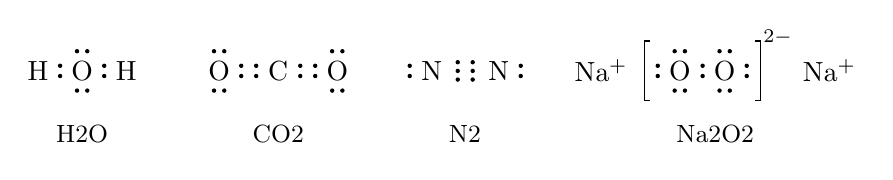
\begin{tikzpicture}[font=\normalsize]
% H2O
\czeroAt{0}{0}{H}{0}{0}{0}{0}\czeroAt{0.56}{0}{O}{2}{2}{2}{2}\czeroAt{1.12}{0}{H}{0}{0}{0}{0}
\node[font=\small] at (0.56,-0.8) {\ce{H2O}};
% CO2
\czeroAt{2.3}{0}{O}{2}{2}{2}{0}\czeroAt{3.05}{0}{C}{0}{2}{0}{2}\czeroAt{3.8}{0}{O}{2}{0}{2}{2}
\node[font=\small] at (3.05,-0.8) {\ce{CO2}};
% N2
\czeroAt{5.0}{0}{N}{0}{0}{0}{2}\czeroAt{5.85}{0}{N}{0}{2}{0}{0}
\foreach \xx in {5.33,5.52} \foreach \yy in {-0.11,0,0.11} \fill (\xx,\yy) circle (0.028);
\node[font=\small] at (5.42,-0.8) {\ce{N2}};
% Na2O2
\node at (7.15,0) {Na$^{+}$};
\czeroAt{8.15}{0}{O}{2}{0}{2}{2}\czeroAt{8.72}{0}{O}{2}{2}{2}{2}
\czeroBr{7.7}{9.17}{$2-$}
\node at (10.05,0) {Na$^{+}$};
\node[font=\small] at (8.6,-0.8) {\ce{Na2O2}};
\end{tikzpicture}}{几种常见物质的电子式\label{fig:00-dots}}

\begin{liti}[基础]
有下列物质：①\ce{MgCl2}；②\ce{H2O2}；③NaOH；④\ce{Na2O2}；⑤\ce{NH4Cl}；⑥\ce{CO2}。其中只含离子键的是\tk，只含共价键的是\tk，含非极性键的是\tk，属于离子化合物的是\tk。
\tcblower
\jie \ce{MgCl2} 由 \ce{Mg^2+} 和 \ce{Cl-} 构成，两个 \ce{Cl-} 之间没有化学键，只含离子键：①。\ce{H2O2}（H—O—O—H）和 \ce{CO2}（O=C=O）只含共价键：②⑥。O—O 键是非极性键，含非极性键的是②④。NaOH 含离子键和 O—H 极性键，\ce{Na2O2} 含离子键和 O—O 非极性键，\ce{NH4Cl} 含离子键和 N—H 极性键，所以离子化合物是①③④⑤。
\end{liti}

\subsection{元素周期律}
同周期主族元素从左到右，电子层数相同，核电荷数逐渐增大，原子核对最外层电子的吸引逐渐增强，原子半径逐渐减小，因此失电子能力减弱、得电子能力增强，即金属性减弱、非金属性增强。同主族元素从上到下，电子层数增多，原子半径增大，原子核对最外层电子的吸引减弱，金属性增强、非金属性减弱。第6章将用电离能、电负性对这些规律作更细致的定量描述。

比较金属性强弱，可以看单质与水或酸反应置换出氢的难易，以及最高价氧化物对应水化物的碱性强弱；比较非金属性强弱，可以看单质与 \ce{H2} 化合的难易、简单氢化物的稳定性，以及最高价氧化物对应水化物的酸性强弱。注意：不能用 HCl 与 \ce{H2S} 水溶液的酸性比较 Cl 与 S 的非金属性，也不能用 HClO 与 \ce{H2SO4} 的酸性比较，因为 HCl、\ce{H2S} 不是含氧酸，HClO 中的 Cl 也不是最高价。

\begin{liti}[典型]
短周期主族元素 X、Y、Z、W 的原子序数依次增大。X 原子最外层电子数是次外层电子数的 2 倍，Y 是地壳中含量最多的元素，Z 的原子半径在短周期主族元素中最大，W 与 Y 同主族。(1) 写出四种元素的符号，并按原子半径由大到小排列。(2) 比较 Y、W 简单氢化物的稳定性。(3) \ce{Z2Y2} 中含有哪些化学键？(4) 比较 X、W 最高价氧化物对应水化物的酸性。
\tcblower
\silu 先由最有特征的信息确定元素，再用周期律比较性质。\\
\jie (1) X 次外层只能是 K 层（2 个电子），最外层 4 个电子，X 为 C；Y 为 O；短周期主族元素中原子半径最大的是 Na，Z 为 Na；W 与 O 同主族且原子序数更大，W 为 S。原子半径：Na$>$S$>$C$>$O（Na、S 同周期，Na 在左；S 比 C、O 多一个电子层；C、O 同周期，C 在左）。(2) 非金属性 O$>$S，稳定性 \ce{H2O}$>$\ce{H2S}。(3) \ce{Na2O2}，含离子键和非极性共价键。(4) 非金属性 S$>$C，酸性 \ce{H2SO4}$>$\ce{H2CO3}。
\end{liti}

% ---------------- 章末 ----------------
\zhangmo{本章小结}
\begin{enumerate}
\item 物质的量把微粒个数与质量、体积联系起来：$n=\frac N{N_\text A}=\frac mM=\frac V{V_\text m}=cV$。$V_\text{m}=22.4$ L·mol$^{-1}$ 只适用于标准状况下的气体。判断 $N_\text{A}$ 的说法时，从物质状态、微粒结构、混合物、溶液中的微粒、电子转移几个角度检查。
\item 离子方程式只写实际参加反应的离子，书写按“写、拆、删、查”进行；判断正误时检查事实、拆分、守恒、用量和反应顺序。离子能否共存，看是否生成沉淀、气体或弱电解质，是否发生氧化还原反应、相互促进的水解或形成配合物，并注意隐含条件。
\item 氧化还原反应的本质是电子转移，特征是化合价升降。氧化剂得电子、被还原，还原剂失电子、被氧化。配平和计算都以得失电子守恒为依据。
\item $A=Z+N$；离子键存在于阴、阳离子之间，共价键是共用电子对；离子化合物的阴离子电子式加方括号并标电荷。同周期从左到右非金属性增强，同主族从上到下金属性增强，比较时要用规定的判断依据。
\end{enumerate}
常见错误有：标准状况下把 \ce{SO3}、HF、\ce{H2O} 当作气体；\ce{Fe^3+} 与 Cu 反应的离子方程式漏配系数，电荷不守恒；用氢化物水溶液的酸性比较非金属性；把 \ce{Na2O2} 中的 \ce{O2^2-} 写成两个 \ce{O^2-}。

\zhangmo{分层练习}
\zu{A组\quad 基础巩固}
\begin{xiti}[start=1]
\item \laiyuan{2025年广东卷第10题}\ 设 $N_\text{A}$ 为阿伏加德罗常数的值。下列说法正确的是\xz
\xxa{1 mol \ce{^{18}O2} 的中子数，比 1 mol \ce{^{16}O2} 的多 $2N_\text{A}$}{1 mol Fe 与水蒸气完全反应，生成 \ce{H2} 的数目为 $2N_\text{A}$}{在 1 L 0.1 mol·L$^{-1}$ 的 \ce{NH4Cl} 溶液中，\ce{NH4+} 的数目为 $0.1N_\text{A}$}{标准状况下的 22.4 L \ce{Cl2} 与足量 \ce{H2} 反应，形成的共价键数目为 $2N_\text{A}$}

\item \laiyuan{原创}\ 下列离子方程式书写正确的是\xz
\xxa{铁与稀盐酸反应：\ce{2Fe + 6H+ = 2Fe^3+ + 3H2 ^}}{\ce{FeCl3} 溶液腐蚀铜板：\ce{Fe^3+ + Cu = Fe^2+ + Cu^2+}}{碳酸钙与醋酸反应：\ce{CaCO3 + 2CH3COOH = Ca^2+ + 2CH3COO- + CO2 ^ + H2O}}{向 \ce{FeBr2} 溶液中通入少量 \ce{Cl2}：\ce{2Br- + Cl2 = Br2 + 2Cl-}}

\item \laiyuan{原创}\ 常温下，下列各组离子在指定溶液中一定能大量共存的是\xz
\xxa{无色溶液中：\ce{K+}、\ce{Cu^2+}、\ce{SO4^2-}、\ce{Cl-}}{pH$=1$ 的溶液中：\ce{Fe^2+}、\ce{NO3-}、\ce{SO4^2-}、\ce{Na+}}{含大量 \ce{Fe^3+} 的溶液中：\ce{NH4+}、\ce{Na+}、\ce{Cl-}、\ce{SO4^2-}}{含大量 \ce{Al^3+} 的溶液中：\ce{Na+}、\ce{HCO3-}、\ce{Cl-}、\ce{SO4^2-}}

\item \laiyuan{原创}\ 下列物质中，既含离子键又含非极性共价键的是\xz
\xx{NaOH}{\ce{Na2O2}}{\ce{NH4Cl}}{\ce{H2O2}}

\item \laiyuan{原创}\ (1) 标准状况下 6.72 L \ce{NH3} 的质量是多少？含多少摩尔 N—H 键？(2) 写出 \ce{MgCl2} 和 \ce{NH3} 的电子式。
\end{xiti}

\zu{B组\quad 高考典型}
\begin{xiti}
\item \laiyuan{原创}\ 已知：①\ce{2Fe^3+ + 2I- = 2Fe^2+ + I2}；②\ce{2Fe^2+ + Br2 = 2Fe^3+ + 2Br-}。(1) 比较 \ce{Br2}、\ce{Fe^3+}、\ce{I2} 的氧化性强弱。(2) 向含 1 mol \ce{FeI2} 的溶液中通入 1.25 mol \ce{Cl2}，写出总反应的离子方程式。

\item \laiyuan{原创}\ 配平：\tk\ce{MnO4-} $+$ \tk\ce{H2C2O4} $+$ \tk\ce{H+} $=$ \tk\ce{Mn^2+} $+$ \tk\ce{CO2 ^} $+$ \tk\ce{H2O}；若反应中转移 0.5 mol 电子，生成标准状况下 \ce{CO2} 多少升？
\end{xiti}

\zu{C组\quad 冲击高分}
\begin{xiti}
\item \laiyuan{原创}\ 设 $N_\text{A}$ 为阿伏加德罗常数的值。下列说法正确的是\xz
\xxa{7.8 g \ce{Na2O2} 中含有的阴离子数为 $0.1N_\text{A}$}{1 mol \ce{Cl2} 与足量 NaOH 溶液反应，转移电子数为 $2N_\text{A}$}{标准状况下，11.2 L \ce{SO3} 中含有的分子数为 $0.5N_\text{A}$}{1 L pH$=1$ 的 \ce{H2SO4} 溶液中含有 \ce{H+} 的数目为 $0.2N_\text{A}$}

\item \laiyuan{原创}\ 向含 0.1 mol \ce{FeBr2} 的溶液中通入 0.1 mol \ce{Cl2}。(1) 写出反应的离子方程式。(2) 被氧化的 \ce{Br-} 占 \ce{Br-} 总量的百分之几？(3) 若改为通入足量 \ce{Cl2}，写出离子方程式。
\end{xiti}

\zhangmo{练习解析}
\begin{jiexilist}
\item \ans{D}A：每个 \ce{^{18}O} 比 \ce{^{16}O} 多 2 个中子，每个 \ce{O2} 多 4 个，1 mol 共多 $4N_\text{A}$；B：\ce{3Fe + 4H2O(g) ->[\text{高温}] Fe3O4 + 4H2}，1 mol Fe 生成 $\frac43$ mol \ce{H2}；C：\ce{NH4+} 与水反应而减少，少于 $0.1N_\text{A}$；D：1 mol \ce{Cl2} 生成 2 mol HCl，形成 2 mol H—Cl 键，正确。
\item \ans{C}A：Fe 与盐酸反应生成 \ce{Fe^2+}；B：电荷不守恒，应为 \ce{2Fe^3+ + Cu = 2Fe^2+ + Cu^2+}；C：碳酸钙难溶、醋酸是弱电解质，都不拆，正确；D：\ce{Fe^2+} 的还原性强于 \ce{Br-}，少量 \ce{Cl2} 先氧化 \ce{Fe^2+}：\ce{2Fe^2+ + Cl2 = 2Fe^3+ + 2Cl-}。
\item \ans{C}A：\ce{Cu^2+} 呈蓝色；B：酸性条件下 \ce{NO3-} 能氧化 \ce{Fe^2+}；C：四种离子与 \ce{Fe^3+} 之间都不反应，可以共存；D：\ce{Al^3+} 与 \ce{HCO3-} 相互促进水解，生成 \ce{Al(OH)3} 沉淀和 \ce{CO2}。
\item \ans{B}NaOH 含离子键和极性键；\ce{Na2O2} 含离子键和 O—O 非极性键；\ce{NH4Cl} 含离子键和极性键；\ce{H2O2} 是共价化合物，不含离子键。
\item (1) $n=\dfrac{6.72}{22.4}=0.300$ mol，$m=0.300\times17=5.1$ g；每个 \ce{NH3} 含 3 个 N—H 键，共 0.90 mol。(2) \ce{MgCl2} 是离子化合物，两个 \ce{Cl-} 分别写在 \ce{Mg^2+} 两侧，各加方括号；\ce{NH3} 是共价分子，N 与 3 个 H 各共用 1 对电子，N 上还有 1 对孤电子对：\\[2pt]
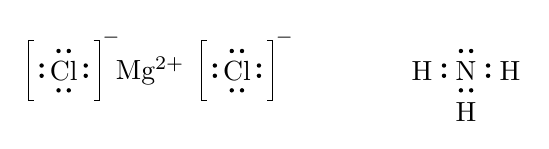
\begin{tikzpicture}[baseline=-3pt]
\czeroAt{0.45}{0}{Cl}{2}{2}{2}{2}\czeroBr{0}{0.9}{$-$}
\node at (1.55,0) {Mg$^{2+}$};
\czeroAt{2.65}{0}{Cl}{2}{2}{2}{2}\czeroBr{2.2}{3.1}{$-$}
\begin{scope}[xshift=5cm]
\czeroAt{0}{0}{H}{0}{0}{0}{0}\czeroAt{0.56}{0}{N}{2}{2}{2}{2}\czeroAt{1.12}{0}{H}{0}{0}{0}{0}\czeroAt{0.56}{-0.52}{H}{0}{0}{0}{0}
\end{scope}
\end{tikzpicture}
\item (1) 由①知氧化性 \ce{Fe^3+}$>$\ce{I2}，由②知 \ce{Br2}$>$\ce{Fe^3+}，所以 \ce{Br2}$>$\ce{Fe^3+}$>$\ce{I2}。(2) 还原性 \ce{I-}$>$\ce{Fe^2+}，\ce{Cl2} 先氧化 2 mol \ce{I-}，消耗 1 mol \ce{Cl2}；剩余 0.25 mol \ce{Cl2} 再氧化 0.5 mol \ce{Fe^2+}。参加反应的 $n(\ce{Fe^2+}):n(\ce{I-}):n(\ce{Cl2})=0.5:2:1.25=2:8:5$，总反应为 \ce{2Fe^2+ + 8I- + 5Cl2 = 2Fe^3+ + 4I2 + 10Cl-}。
\item 2、5、6、2、10、8；11.2 L。Mn 由 $+7$ 价降为 $+2$ 价，每个得 5 个电子；C 由 $+3$ 价升为 $+4$ 价，每个 \ce{H2C2O4} 失 2 个电子。最小公倍数 10，所以 \ce{MnO4-} 配 2，\ce{H2C2O4} 配 5，\ce{CO2} 配 10；由电荷守恒，左边 $-2+x=+4$，\ce{H+} 配 6；最后由 H 守恒得 8 个 \ce{H2O}。生成 10 mol \ce{CO2} 转移 10 mol 电子，转移 0.5 mol 电子时生成 0.5 mol \ce{CO2}，标准状况下为 11.2 L。
\item \ans{A}A：7.8 g \ce{Na2O2} 为 0.1 mol，含 0.1 mol \ce{O2^2-}，正确；B：\ce{Cl2 + 2NaOH = NaCl + NaClO + H2O}，1 个 \ce{Cl2} 中一个 Cl 得 1 个电子、另一个失 1 个电子，1 mol \ce{Cl2} 转移 1 mol 电子；C：标准状况下 \ce{SO3} 不是气体；D：pH$=1$ 时 $c(\ce{H+})=0.1$ mol·L$^{-1}$，1 L 中 \ce{H+} 为 $0.1N_\text{A}$，pH 已经反映了 \ce{H+} 的总浓度，不能再乘 2。
\item (1) \ce{2Fe^2+ + 2Br- + 2Cl2 = 2Fe^3+ + Br2 + 4Cl-}。还原性 \ce{Fe^2+}$>$\ce{Br-}，0.1 mol \ce{Fe^2+} 先消耗 0.05 mol \ce{Cl2}，剩余 0.05 mol \ce{Cl2} 氧化 0.1 mol \ce{Br-}；参加反应的 \ce{Fe^2+}、\ce{Br-}、\ce{Cl2} 物质的量之比为 $1:1:1$。(2) $\dfrac{0.1\ \text{mol}}{0.2\ \text{mol}}=50\%$。(3) \ce{Cl2} 足量时 \ce{Fe^2+} 和 \ce{Br-} 全部被氧化，二者按 \ce{FeBr2} 的组成 $1:2$ 参加反应：\ce{2Fe^2+ + 4Br- + 3Cl2 = 2Fe^3+ + 2Br2 + 6Cl-}。
\end{jiexilist}
